\chapter{腹膜后腔}

\section{检查方法}

\subsection{扫描前准备}

扫描前的准备与腹部其他部位大致相同。扫描前空腹4~6小时,扫描前1小时口服1.5%~2.0%的复方泛影葡胺800~1000ml,扫描前15分钟再服300ml。尤其对儿童和成人消瘦病例肠道准备尤为重要。

\subsection{扫描方法}

由于腹膜后间隙范围广,上起膈下,下与盆腔筋膜间隙相通,因此扫描范围应足够宽大。扫描一般从剑突向下至髂嵴水平。层厚10mm,间隔为10mm或20mm,必要时加薄层扫描。为了显示中线区域大血管及周围间隙,必要时可做增强扫描。腹膜后间隙中诸筋膜、间隙对诊断疾病和认识其扩散情况具有重要价值,为了有利于显示它们,窗宽宜稍宽、窗位宜稍低,必要时可做三维、冠状或矢状重建。

\section{正常解剖及变异}

\subsection{腹膜后腔内包含的组织和器官}

腹膜后腔是后腹膜与腹后壁腹横筋膜之间解剖间隙及其解剖结构的总称。

该间隙上达膈肌,下至盆腔入口。其内除疏松结缔组织和筋膜外,还包含一些器官和结构,如肾、输尿管、肾上腺、胰腺、十二指肠降部、部分升结肠和降结肠,以及腹主动脉及其分支、下腔静脉及其属支、淋巴管、淋巴结和神经等。在肾脏水平被分为肾旁前间隙、肾周间隙和肾旁后间隙(图\ref{fig19-1})。

\begin{figure}[!htbp]
 \centering
 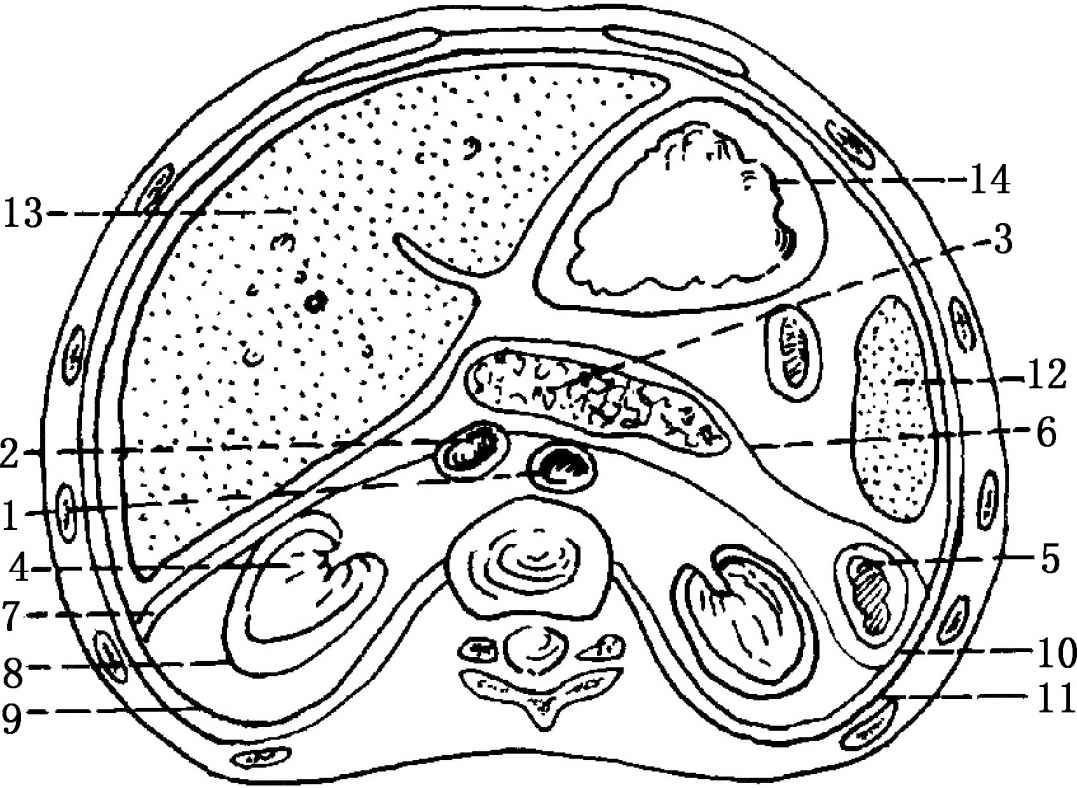
\includegraphics[width=.7\textwidth,height=\textheight,keepaspectratio]{./images/Image00381.jpg}
 \captionsetup{justification=centering}
 \caption{腹膜后腔的正常解剖\\{\small 1.主动脉;2.下腔静脉;3.胰腺;4.肾;5.降结肠;6.腹膜;7.前肾筋膜;8.肾包膜;9.后肾筋膜;10.侧锥筋膜;11.横筋膜;12.脾;13.肝;14.胃}}
 \label{fig19-1}
  \end{figure} 

\subsection{肾旁前间隙}

该间隙为后腹膜与前肾筋膜之间的区域,外侧受限于侧锥筋膜。其内包含升、降结肠,十二指肠降段、水平段及升段,以及胰腺、肠系膜血管等。解剖学上小肠系膜和横结肠系膜根部,均与此间隙相通连。

可知:①在胰腺平面两侧肾旁前间隙潜在相通。②由于肾前筋膜在肾上腺上方与肾后筋膜相融合,而后再融合于膈肌筋膜,故此间隙上方可达膈肌筋膜前方。③下方于髂嵴稍下平面,可以与肾周间隙、肾旁后间隙相通。

\subsection{肾周间隙}

该间隙位于肾前、后筋膜之间,形似倒置的锥体,内有肾上腺、肾、输尿管和出入肾门的血管,以及较丰富的肾周脂肪组织(脂肪囊)。

可知:①在内侧,肾前筋膜融汇于肠系膜根部及胰腺、十二指肠后方的围绕大血管的致密结缔组织中。②肾后筋膜则融合于腰大肌或腰方肌筋膜(但也有学者认为不附着于腰大肌)。③肾周间隙像个倒立的圆锥。其下端,肾前后两层筋膜松散的融合在髂筋膜及居内侧的输尿管周围结缔组织中,多认为该间隙下端是向髂凹开通的。④上端止于膈筋膜。

\subsection{肾旁后间隙}

该间隙位于肾后筋膜后方与腹后壁腹横筋膜之间,其内包含脂肪组织及血管、淋巴管,无脏器。

该间隙内侧止于肾后筋膜与腰肌筋膜融合处;外侧与腹侧壁的腹膜外脂肪层相通连,并进而通过腹前壁的腹膜外脂肪使两侧在前方潜在的相通;下方与盆外筋膜间隙相通,在髂嵴平面以下,同时也潜在的与肾旁前间隙和肾周间隙相通;上方,肾旁后脂肪层向上伸延而构成属于腹膜外脂肪的一薄层膈下脂肪。

国外有学者认为,肾后筋膜内侧附着于腰方肌浅面,它可以附着于腰方肌的内侧、中间或外侧,但并不是附着在腰大肌的筋膜上。因此肾旁后间隙的内侧界并不非常靠内侧。这表明腰大肌前方与肾周间隙直接相邻,这是部分肾癌可以直接侵犯腰大肌的解剖学依据。

\subsection{肾周间隙与周围通连关系的新观点}

1.肾周间隙的内侧通连:情况复杂,分歧较多,有以下多种学说。①两侧肾周间隙内侧自由交通;②两侧肾周间隙的某些部位相交通;③两侧肾周间隙不相通;④其他。

2.肾周间隙的外侧通连:一般认为肾前、后筋膜于外侧方融合成侧锥筋膜,呈封闭状。

3.肾周间隙的上方通连:肾周间隙上方的解剖叙述与肝裸区的关系是有争议的,目前有两种观点。①肾前、后筋膜在肾上腺上方牢固地融合,并固定于膈筋膜上,故肾周间隙上方呈封闭状态。因此不与肝裸区相通。②有些学者认为右侧肾周围间隙上方与肝裸区相通连;左侧肾周间隙与邻近左膈下腹膜外间隙(胃裸区)间有自由交通。

4.肾周间隙的下方通连:肾周间隙向下开放与否,尚未达成一致意见。①下方开放;②下方关闭;③其他:有学者提出虽然肾周间隙是密闭的,但液体可通过肾周间隙的桥隔漏出,延伸到筋膜间平面,进而到达盆腔。

\subsection{肾周间隙内的桥隔}

肾周间隙长期以来一直被认为是充满脂肪的区域。但近些年来认为其内还存在着纤维结缔组织形成的桥隔。根据桥隔的走行可分为3组:①连接在肾包膜与肾筋膜之间;②附着在肾包膜上,其走行基本上平行于肾表面的肾-肾桥隔;③连接在肾前、后筋膜之间。

国外有学者认为,CT图像上最常见的是沿后外侧肾包膜走行的背侧肾-肾桥隔。并指出肾周间隙内的桥隔成为疾病在肾与肾筋膜平面之间蔓延的通道。此外,桥隔也可能是导致肾周间隙炎症、出血等局限化的重要解剖基础。

\subsection{肾筋膜}

肾筋膜在CT扫描中,正常厚约1~2mm。大于2~3mm或局限性增厚,应视为异常。

近些年来通过大量的研究证实,肾筋膜并不是单层的膜结构,而是分层的,并多认为分两层。还有学者从胚胎发育的角度提出,肾筋膜不是由一单层膜构成,而实际上可能是在胚胎发育时遗留下的胚胎肠系膜相互融合形成的分离的多层膜结构。亦有学者用组织学、间隙灌注、断面解剖和CT扫描的方法证实肾后筋膜分为内(前)、外(后)两层,内(前)层与肾前筋膜相延续,外(后)层续侧锥筋膜。因而,肾旁前间隙有水肿或炎症时,可以直接通过该前、后层之间而达到肾脏的后外方,这在急性胰腺炎腹膜后扩展型沿此解剖变异扩散时表现尤为明显。

\subsection{后腹膜反褶变异}

国外有学者提及后腹膜反褶变异,即后腹膜在外侧绕过结肠前面以后未直接与侧腹壁腹膜相延续,而是反褶向后直至肾后,然后再折回与侧腹膜相延续,从而导致腹膜腔向肾后伸展。这在腹腔积液时尤其明显。腹腔积液可到达肾脏的后外1/3或更向内到达腰大肌处。除腹腔积液以外,有时小肠亦可伸入其中。

\subsection{腰肌}

腰肌由腰大肌、腰小肌和髂肌组成。腰方肌属于腹肌的后群,位于腰大肌的外后侧,起自髂嵴,止于12肋,不属于腰肌的组成部分。而腰肌属于下肢肌中髋肌前群范畴。

1.腰大肌:起自T\textsubscript{12} ~L\textsubscript{4}
椎体侧面和所有腰椎的横突,向下与髂肌联合成髂腰肌,在腹股沟韧带下方通过,止于股骨小转子。

CT表现为腰椎旁成对的软组织影,从头端至尾端其形状由三角形变为圆形,体积亦逐渐变大。神经肌肉失调可致腰肌萎缩变小,并可见到部分肌肉组织被脂肪代替所形成的较低密度。

2.腰小肌:细而长,位于腰大肌前方,在人类它的出现率为50%。

CT表现,如腰小肌存在,可见在腰大肌前方见小而圆的软组织块影,勿误认为增大的淋巴结。由于先天发育和运动习惯不同,两侧腰小肌可大小不对称。

3.髂肌:位于髂窝内,与该窝形状相似,为扇形扁肌。绝大部分起自髂窝,部分起自髂筋膜、髂前下棘和骶骨翼。肌束向下逐渐集中,部分肌纤维编入腰大肌,部分纤维止于股骨小转子及髋关节囊。CT表现为髂窝内软组织块影。

此外,有时可见交感神经干、腰动脉和腰静脉呈小的软组织密度影,位于腰大肌内侧与腰椎之间。

\section{腹部大血管疾病}

\subsection{腹主动脉病变}

\subsubsection{动脉粥样硬化}

\textbf{【CT表现】}
包括动脉壁的钙化、管腔的轻度扩张和扭曲、粥样斑块或血栓形成,以及血管腔狭窄乃至完全闭塞。增强扫描粥样斑块或血栓形成呈沿腔内壁分布的斑块状或环形低密度充盈缺损,血管闭塞时增强扫描无强化。

\textbf{【鉴别诊断】}
当明显迂曲时应注意与腹主动脉瘤相鉴别。当以管腔狭窄为主时,须与大动脉炎相鉴别,后者主要见于年轻人,CT可见明显增厚的管壁及向心性狭窄的管腔。

\subsubsection{真、假性主动脉瘤及主动脉夹层}

(见第十章第四节)。

\subsubsection{主动脉瘤术后并发症}

包括出血、感染、假性动脉瘤形成、主动脉-十二指肠瘘,以及主要血管或人造血管支的闭塞等。

\subsection{下腔静脉先天性发育异常}

大部分下腔静脉先天发育异常或畸形无临床症状和体征,少数伴其他畸形。

\subsubsection{下腔静脉肝段缺如伴奇静脉或半奇静脉的连接}

\textbf{【病因】}
在胚胎第6周,下腔静脉干与肝静脉干连接失败,血液从后肾段经过奇静脉或半奇静脉回流入心脏,肝静脉直接回流入右房。下腔静脉在肾静脉和肝静脉之间缺如,这种畸形可孤立发生,也可伴先心病、多脾或腹部内脏转位等。

\textbf{【CT表现】}
正常下腔静脉的肝段部位缺如,在右膈脚后主动脉右侧,增宽的奇静脉表现为孤立性圆形阴影,或者膈脚后主动脉两侧可见增宽的奇静脉和半奇静脉影,须注意与增大淋巴结鉴别。

\subsubsection{下腔静脉易位}

又称左位下腔静脉。

\textbf{【病因】}
在胚胎期,右静脉干异常退化,而左静脉干持续存在,形成该畸形。

\textbf{【CT表现】}
可见单个下腔静脉自脊柱左侧上升;在肾静脉水平,下腔静脉跨过主动脉的前方或后方,再沿脊柱右侧上升,进入右房。

\subsubsection{双下腔静脉}

又称下腔静脉重复畸形。

\textbf{【病因】}
在胚胎期,如左主静脉肾下段未退化,而与右主静脉一起发育,则形成该畸形。

\textbf{【CT表现】}
于肾静脉下方脊柱左、右侧各见一条下腔静脉。左右两支直径可以相等,或其中一支为主要血管,通常左侧较粗。在肾静脉水平上方直至横膈,仅见右侧单一的下腔静脉。

\textbf{【鉴别诊断】}
左侧下腔静脉追踪至髂总静脉水平,以此可与扩张的左侧生殖腺静脉相鉴别,后者扩张的血管可追踪至腹股沟水平。

\subsubsection{腔静脉后输尿管}

又称环腔静脉输尿管(详见第十五章第三节)。

\subsection{下腔静脉的癌栓和血栓形成}

癌栓或血栓是下腔静脉梗阻的常见原因。

\textbf{【病因】}
可累及下腔静脉的癌肿包括肾癌、肾上腺肿瘤、腹膜后肉瘤、肝细胞癌、淋巴瘤等。肝癌虽可侵及下腔静脉,但不如侵及门脉系统常见。

\textbf{【CT表现】}
血栓或癌栓它们都表现为腔内充盈缺损和局部管腔扩大,较难鉴别。①增强前癌栓的密度通常比周围血液密度低;新鲜血液形成的血栓密度与循环血液类似;而陈旧性血栓的密度则低于周围血液。②增强扫描癌栓和血栓均呈低密度的充盈缺损。下腔静脉癌栓可表现为低密度充盈缺损的周边密度增高,可能是下腔静脉壁的血管强化或肿瘤血管导致的癌栓强化。③有的病例肿瘤癌栓可伸展超出下腔静脉壁的范围,有助于明确诊断。④下腔静脉完全阻塞者,可显示广泛侧支循环。

此外,下腔静脉瘤时,其内可见低密度血栓及血栓钙化,但下腔静脉显著扩张有助于下腔静脉瘤的诊断。

\subsection{下腔静脉平滑肌肉瘤}

原发性血管肿瘤极为罕见,主要发生在大的静脉,尤其下腔静脉较常见;动脉肿瘤占20%以下,且多为恶性。下腔静脉的原发性肿瘤以平滑肌肉瘤较常见。

\textbf{【临床表现】}
多见于60岁以上女性,其临床症状与下腔静脉梗阻的水平、程度,以及受累的输入血管有关,当向腔外生长时多无症状。

\textbf{【CT表现】}
无特异性,可显示肿瘤的部位、长度、侵犯壁外的范围及与邻近器官的关系和侧支循环等。由于平滑肌肉瘤为少血管肿瘤,增强扫描多无明显强化。总之,CT对下腔静脉肿瘤诊断的敏感性高,特异性差。

\section{腹膜后腔炎症及脓肿}

腹膜后间隙炎症和脓肿在临床上一般均有感染的症状,如发热、腰胁部疼痛甚至叩击痛,化验检查白细胞和中性粒细胞升高。尿液检查若无肾脏本身病变存在,一般无阳性发现。

\subsection{肾旁前间隙炎症及脓肿}

\textbf{【病因】}
该间隙的炎症和脓肿主要来源于急性胰腺炎和十二指肠、升结肠、降结肠向腹膜后腔穿孔等。穿孔原因可以是外伤、肿瘤坏死以及肠炎等。比较少见的来源还有腹膜后位阑尾的急性炎症穿孔;以及肝脓肿溃入肝裸区,然后再向下进入腹膜后其他间隙等。最常见的是急性胰腺炎及其胰周受累和脓肿形成。

\textbf{【CT表现】}
受累的肾旁前间隙脂肪组织密度增高,呈不规则的片状、斑片状或条索状。如病灶内有气泡或气液平面,则脓肿的诊断相对无疑。若无脓腔存在,仅表现为局限性积液,或者并有脓肿壁强化的表现,结合临床表现也可考虑脓肿的可能性。

此外,还具有以下特点。①由于该间隙有较疏松的脂肪组织,因此易发生蜂窝组织炎,其脂肪组织密度增大呈液体或近似软组织密度。水肿范围较宽,常界限不清。即使脓肿已形成,其脓肿壁有时也不大完整。有气体积存时,气体分布较弥散。②发生于胰周者,胰周脂肪的改变可主要出现于胰前或胰后。③发生于十二指肠、升结肠、降结肠腹膜后段后方者,通常可见该肠段后方的脂肪组织有前述改变,并显示肠管与前肾筋膜间距增宽(一般正常时,均很靠近)、肠后壁受压前移,这一点对确定病变是否处于肾旁前间隙甚为重要。④肾前筋膜通常均有增厚。

\subsection{肾周间隙炎症及脓肿}

\textbf{【病因】}
其最常见的原因为肾脓肿穿破或肾盂肾炎所继发。其他少见原因有血源性肾周感染、急性胰腺炎腹膜后间隙扩散所继发、肾破裂继发感染等。肾周间隙内的桥隔在一定程度上限制了炎症在肾脂肪囊内的扩散并有利于炎症的局限化或分隔化。

\textbf{【CT表现】}
肾脂肪囊内桥隔有不规则增粗;脂肪组织内可见斑片状、条索状高密度区,也可呈水样或软组织密度。当有脓肿形成时,其内密度较均匀,脓肿壁亦较清晰。若脓腔内有气体则可显示气液平面或气泡。增强扫描脓肿壁常有强化,且有利于显示肾实质内的病灶。脓肿自溃或扩散可见到腹后壁、肾旁后间隙、腰大肌相邻处的炎症或脓肿(图\ref{fig19-2}),相邻肾筋膜可增厚。

\begin{figure}[!htbp]
 \centering
 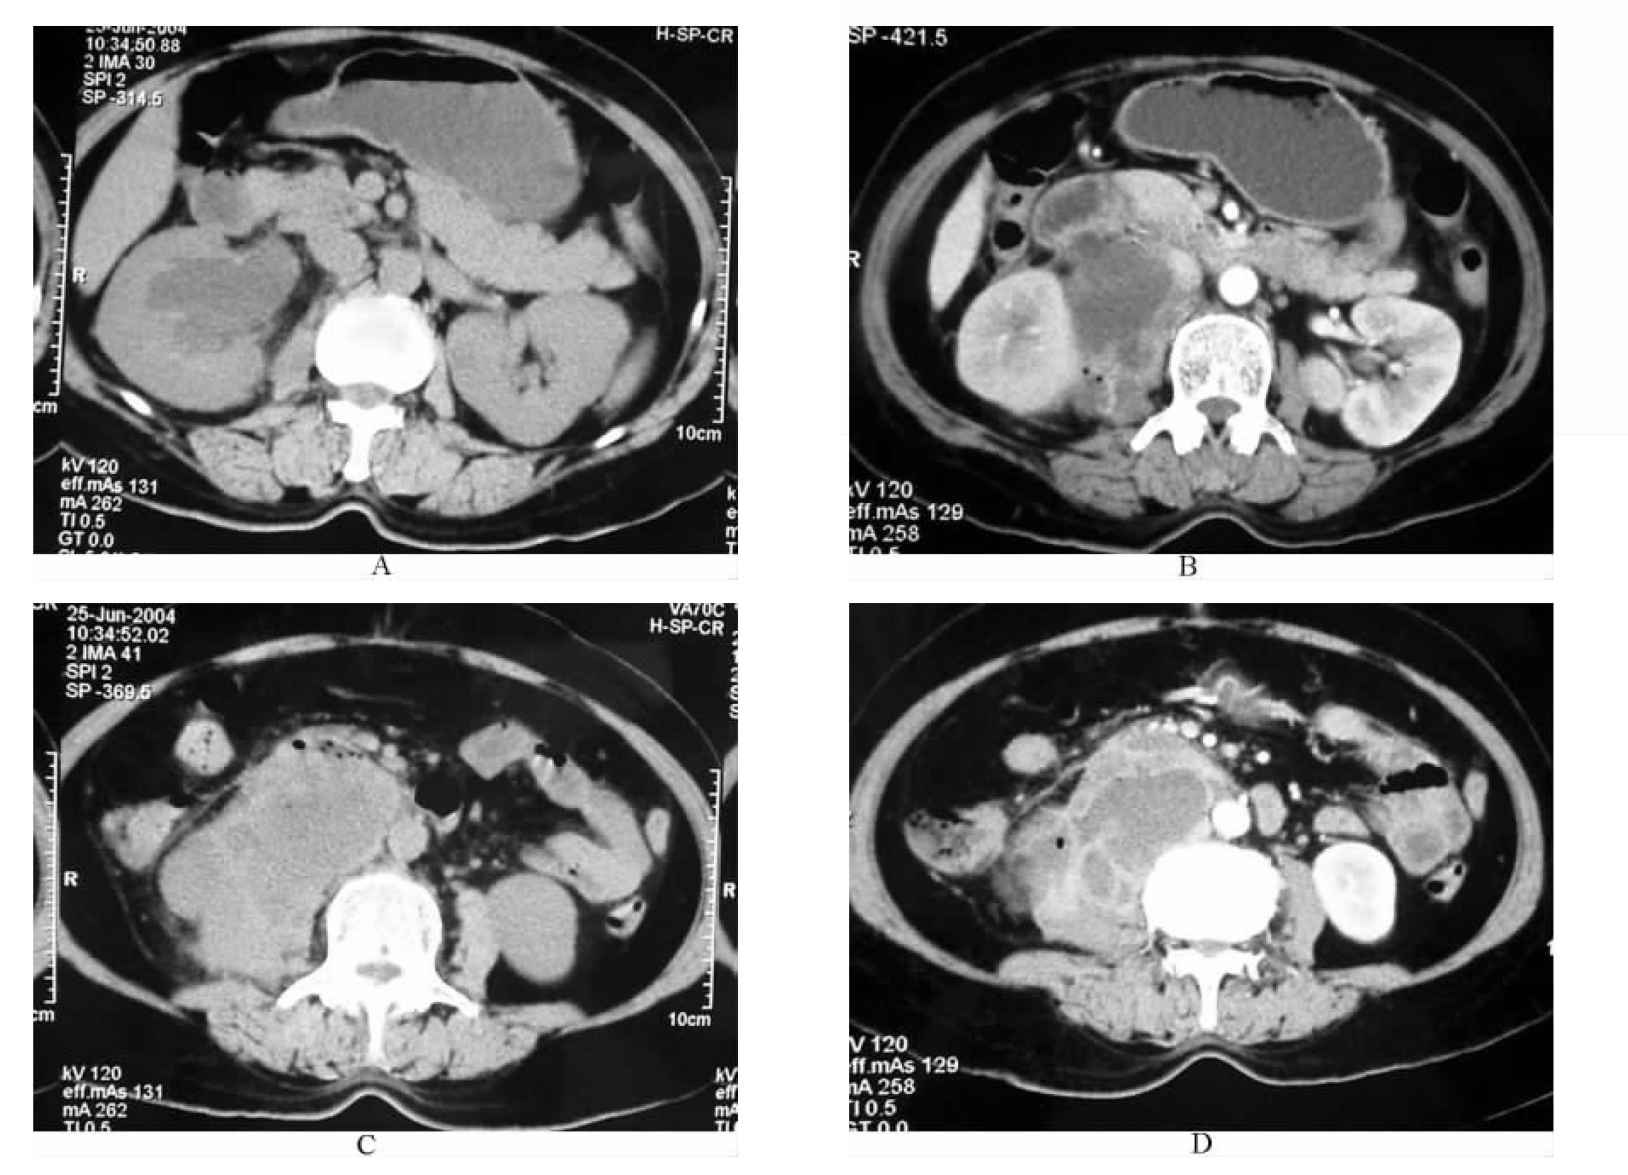
\includegraphics[width=.7\textwidth,height=\textheight,keepaspectratio]{./images/Image00382.jpg}
 \captionsetup{justification=centering}
 \caption{右肾积水尿液外渗并腹膜后脓肿形成\\{\small 涉及腹膜后各间隙和腰大肌(B、D为增强扫描)}}
 \label{fig19-2}
  \end{figure} 

\subsection{肾旁后间隙炎症及脓肿}

\textbf{【病因】}
该间隙内主要是脂肪组织,其炎症主要是继发的,可来源于急性胰腺炎的跨筋膜间隙和腹膜后间隙扩散,也可来源于肾周间隙炎症或后腹壁炎性病变,以及腰大肌脓肿的直接扩散。此外,盆壁、髂窝炎症和脓肿,沿盆腔筋膜间隙、髂窝区域腹膜外间隙向上扩散也可达此间隙。

\textbf{【CT表现】}
肾旁后间隙脂肪密度增高,呈不规则斑片状或条索状,界限模糊。该间隙可相应增宽。当脓肿形成时,可显示脓腔及脓肿壁。相邻肾后筋膜可增厚,腹壁亦可有水肿增厚。

\section{腹膜后腔肿瘤}

\subsection{概述}

\subsubsection{原发性腹膜后肿瘤的分类}

原发性腹膜后肿瘤相对少见,但种类繁多,可来源于多种组织(见表\ref{tab19-1})。腹膜后肿瘤以恶性多见,约占80%。

\begin{table}[htbp]
\centering
\caption{原发性腹膜后肿瘤的病理分类}
\label{tab19-1}
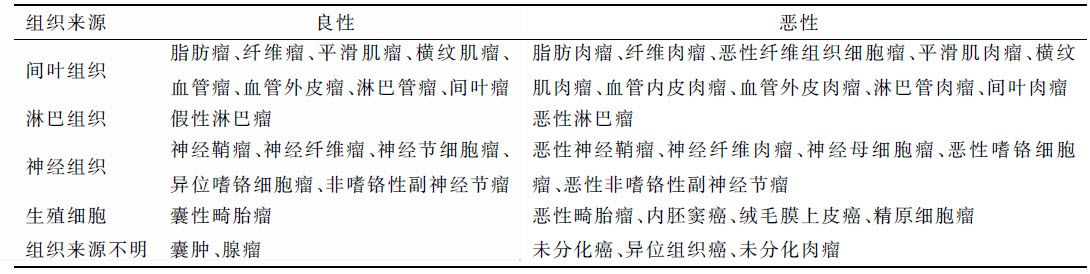
\includegraphics[width=\textwidth,height=\textheight,keepaspectratio]{./images/Image00383.jpg}
\end{table}

1.恶性肿瘤:多起源于中胚层组织,以脂肪肉瘤、平滑肌肉瘤、恶性纤维组织细胞瘤、纤维肉瘤、恶性畸胎瘤、淋巴瘤等较常见。此外,还较常见的有神经纤维肉瘤、神经母细胞瘤、横纹肌肉瘤、血管肉瘤等。

2.良性肿瘤:很少见,包括脂肪瘤、平滑肌瘤、畸胎瘤、异位嗜铬细胞瘤、神经纤维瘤、神经鞘瘤、神经节细胞瘤、血管瘤及淋巴管瘤等。

\subsubsection{腹膜后良、恶性肿瘤的CT特点}

其CT特点为多数良性肿瘤边界清晰,形态规则,与周围脏器少有粘连,无侵犯表现。恶性肿瘤则多有周围脏器的粘连与侵犯,边界不清,形态不规则或呈多结节融合。此外,国内有学者认为,囊性均为良性,囊实性及实性良恶性均可见。总之,良、恶性肿瘤的鉴别着重于肿块的边界、形态及与周围脏器的关系,而体积大小及是否有出血、坏死、囊变对良恶性的鉴别价值有限。

\subsection{腹膜后脂肪肉瘤}

脂肪肉瘤是腹膜后最常见的原发恶性肿瘤。

\textbf{【病理】}
有5种亚型。Ⅰ型:分化好的脂肪肉瘤(又分为脂肪瘤样脂肪肉瘤、硬化性脂肪肉瘤);Ⅱ型:黏液性脂肪肉瘤;Ⅲ型:多形性脂肪肉瘤;Ⅳ型:圆细胞性脂肪肉瘤;Ⅴ型:去分化脂肪肉瘤。其中Ⅰ、Ⅱ型属低度恶性,后3型属高度恶性肿瘤。不同组织学亚型的脂肪肉瘤其共同点在于瘤内发现不同分化阶段的脂肪母细胞。

\textbf{【临床表现】}
早期无明显症状,主要表现为腹胀、腹部不适、腹部包块,部分有腹痛,还可有消瘦、大便困难等,少数病例为体检发现。

\textbf{【CT表现】}
由于肿瘤内脂肪细胞的分化程度、纤维组织或黏液性组织混合程度不同而有不同的CT表现。国外有学者将其分为3型:

1.实体型:肿瘤分化不好,肿瘤内成分以纤维组织为主,肿瘤CT值>20Hu。

2.假囊肿型:为黏液性脂肪肉瘤。肿瘤似囊性病变,水样密度,CT值在-20Hu与20Hu之间,密度均匀。

3.混合型:肿瘤内成分以纤维组织为主伴散在的脂肪组织。肿瘤密度不均,实质部分CT值>20Hu,而脂肪灶处CT值<-20Hu。

此外,本病具有侵袭性生长方式,它可伸入各间隙内。增强扫描可有均匀或不均匀强化,并可见坏死、囊变表现。国内有学者报道,去分化脂肪肉瘤早期中度或显著不均匀强化,并有延迟强化。

\textbf{【鉴别诊断】}
如发现瘤内含有脂肪密度,结合其他表现多可确定脂肪肉瘤。①分化不良的实体型不易与其他肿瘤相鉴别,甚至病理也不易与纤维肉瘤区分,而划为纤维脂肪肉瘤。②如发现瘤内含有与水密度近似的区域,同时有侵犯征象,则提示本病,且多为假囊肿型,但难以与其他肿瘤坏死、囊变相鉴别。③分化良好的脂肪肉瘤与良性脂肪瘤相似,难以鉴别,但脂肪瘤密度均匀无强化。④少数可有钙化,应注意与畸胎瘤鉴别。

\subsection{常见的原发恶性腹膜后肿瘤}

仅就其CT特点简述如下:

1.脂肪肉瘤:(见前述)。

2.平滑肌肉瘤:①病灶中心多有广泛和不规则的水样坏死、囊性变区。如有出血呈高密度区,通常无钙化。②增强后边缘性环状强化,如坏死区很大呈厚壁囊肿样改变。③肝脏是最常见的转移部位,可形成典型的“牛眼征”,亦可转移到肺、肠系膜、网膜等处。坏死囊变还可见于其他肿瘤如神经鞘瘤、精原细胞瘤等。

3.恶性纤维组织细胞瘤:好发于四肢及腹膜后腔。CT表现为软组织肿块,其中有低密度坏死区,约1/4病例见肿瘤内或周边无定形钙化,增强扫描可有不规则强化。

4.神经母细胞瘤:见于婴幼儿或儿童,伴腹痛、腹块。CT表现为腹膜后分叶状肿块,肿块内有斑点状钙化,并可见腹主动脉及其分支的包埋等征象。

5.横纹肌肉瘤:CT表现为软组织肿块及其坏死区。

6.异位恶性嗜铬细胞瘤:肿瘤主要沿主动脉旁交感神经节分布,分功能性和无功能性。一般恶性者生长较大,且常有坏死,边缘不清,可有钙化。大多血供丰富而强化显著。

\subsection{常见的原发良性腹膜后肿瘤}

仅就其CT特点简述如下:

1.囊肿:表现为轮廓完整、边界清晰、无强化的水样密度病灶,有均匀薄壁(图\ref{fig19-3}A)。

2.乳头状腺瘤:薄壁囊性病变,伴强化的壁结节。

3.脂肪瘤:呈脂肪密度,密度均匀,可有部分纤维隔。边缘清楚,无强化。

4.畸胎瘤:大多为良性,恶性者不足1%。由于含有3种胚层组织,故肿瘤内含有骨组织、软组织、液体、脂肪和毛发等不同成分,CT可予显示(图\ref{fig19-3}B)。其实质部分可强化,囊性部分呈低密度。由于肿瘤内脂肪成分有限,CT常不能显示脂肪的存在,如发现有多种不同密度的成分混合存在则有助于诊断。毛发呈球状,往往漂浮在脂肪和(或)液体成分的表面称为“漂浮征”。肿瘤周边钙化,常呈“蛋壳”样。

\begin{figure}[!htbp]
 \centering
 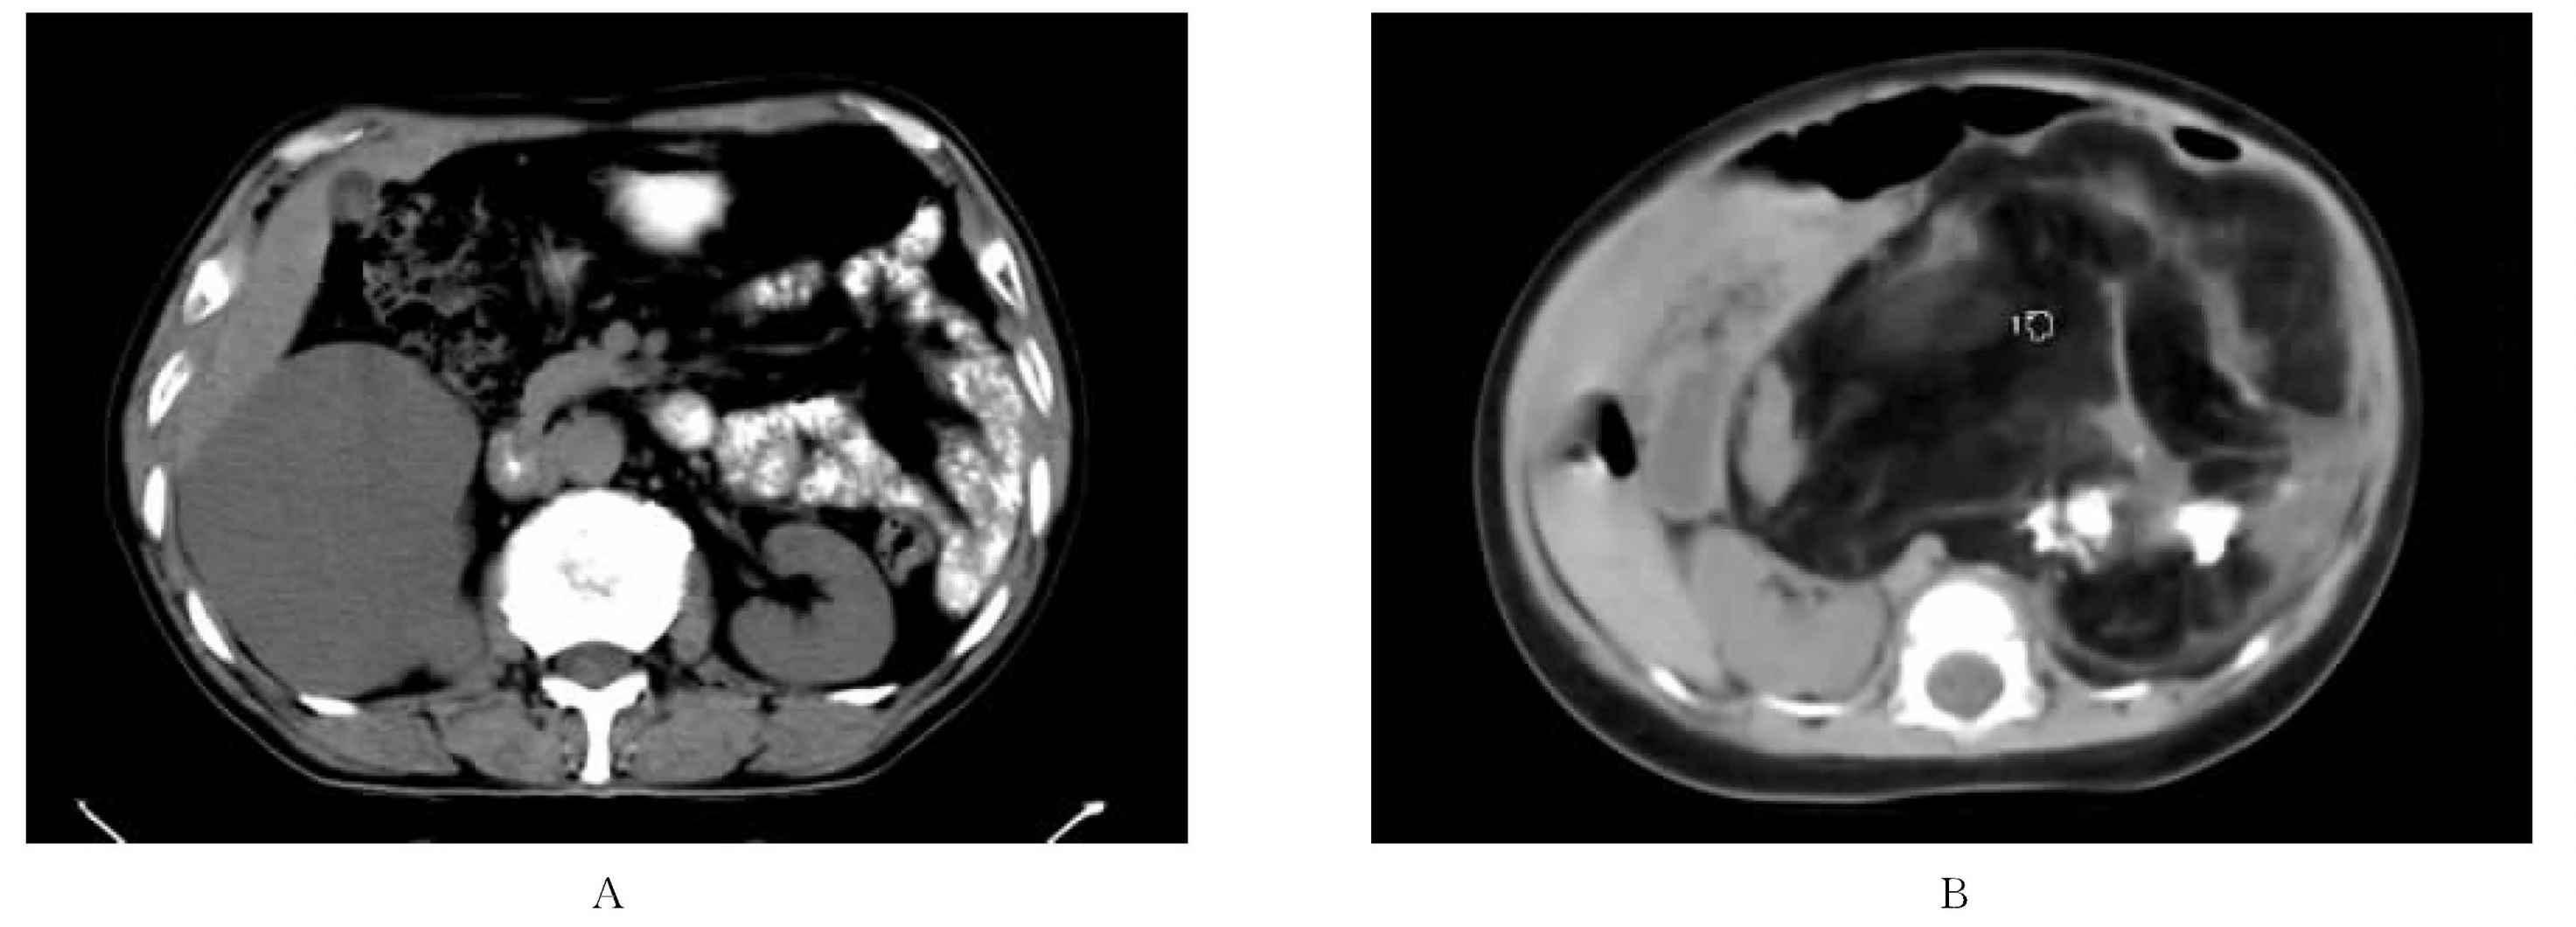
\includegraphics[width=.7\textwidth,height=\textheight,keepaspectratio]{./images/Image00384.jpg}
 \captionsetup{justification=centering}
 \caption{腹膜后良性肿瘤\\{\small A.囊肿:右侧腹膜后有巨大水样密度灶,边缘光滑锐利;B.畸胎瘤:腹膜后有巨大混杂密度肿块,其内含有大量脂肪,并含有软组织密度灶和高密度骨组织,胃肠道受压前移、右肾受压变形}}
 \label{fig19-3}
  \end{figure} 

5.良性平滑肌瘤:一般密度均匀、边缘光整,强化显著,有一定特点,但有时肿瘤中心亦可坏死。

6.良性神经源性肿瘤:是最常见的良性腹膜后肿瘤。①肿瘤多位于脊柱两侧,呈圆形或椭圆形,边缘清晰,包膜完整。②肿瘤可巨大,>5cm的肿块常密度不均,可有实质斑块状钙化或包膜斑点状钙化。增强扫描均匀或不均匀强化,常见周围强化明显,中央见低密度的坏死或囊变区。③<5cm者平扫及增强多密度均匀。

此外,纤维瘤、横纹肌瘤等良性肿瘤并无特异性CT表现。异位良性嗜铬细胞瘤沿脊柱两侧分布,功能性者结合临床不难诊断,无功能性者肿块多较大,CT诊断困难。

\subsection{小结}

\subsubsection{腹膜后肿瘤的CT分析}

1.肿块与腹腔后器官关系密切、邻近大血管移位、变形及腹后壁和(或)盆壁受侵是腹膜后肿瘤的定位依据。

2.良、恶性肿瘤的鉴别主要依据肿块的边缘、形态及与周围脏器的关系(亦非绝对)。而体积大小、是否有钙化、囊变等对鉴别价值有限。

3.脂肪瘤呈典型脂肪密度肿瘤,如脂肪内存在不均匀间隔线或软组织成分,则应考虑脂肪肉瘤。实体型或假囊肿型脂肪肉瘤诊断较困难。

4.平滑肌肉瘤多有大片坏死区,包括其转移灶内也有坏死区,且不伴钙化。但坏死、囊变也可见于其他肿瘤如神经鞘瘤。

5.畸胎瘤多为良性,呈多种成分的囊实性肿块。

6.神经源性肿瘤多为良性,且年龄偏小,肿瘤位置偏向中线沿脊柱两侧,密度均匀或不均。如神经鞘瘤产生黏液性变可极似囊肿,但CT值高于水。

7.婴幼儿和儿童患者软组织肿块内有钙化者,以神经母细胞瘤可能性大。

8.主动脉旁肿块,如有阵发性高血压,血中VMA和儿茶酚胺浓度升高,则异位嗜铬细胞瘤可明确诊断。但无功能性者诊断困难。

9.肿瘤内出现钙化以恶性纤维组织细胞瘤最常见,亦可见于神经母细胞瘤、畸胎瘤、异位嗜铬细胞瘤、海绵状血管瘤,甚至脂肪肉瘤等。

10.淋巴结增大广泛,涉及腹膜腔、腹膜后,并有融合表现,为恶性淋巴瘤的特点。而淋巴结转移瘤通常为不连续的结节状病变,但有时鉴别困难。

11.薄壁囊状肿块,内容物近似水,囊壁极薄,为囊肿的特点。

12.肿块强化显著者,倾向于血管源性肿瘤(且其持续时间长)及化学感受器瘤,其次是嗜铬细胞瘤。

\subsubsection{腹膜后肿瘤的定位诊断及与肠系膜肿块的鉴别}

1.肿块与腹膜后器官如肾、输尿管、腰大肌等关系密切,肾输尿管受压移位、肾周脂肪轮廓消失、胰腺和肠管向前推移。

2.邻近大血管移位、变形,可见腹主动脉、下腔静脉、肾静脉等受压推移或被肿瘤包埋。

3.邻近腹后壁和(或)盆壁界限不清或消失。

4.肿块径线较大,常常>7cm。因腹膜后肿瘤只有达到一定大小时才会压迫和推移邻近器官而产生腹块、腹痛及其他相应症状,所以第一次就诊时肿瘤多较大。

在定位诊断时主要应与肠系膜肿块相鉴别。后者与肠管关系密切、肠道包绕或紧贴肿块,常使肠管以肿块为中心向两侧推移,而腹膜后肿块只使肠管前移。另外肠系膜肿瘤可使肠系膜血管受压前移或后移,而腹膜后肿瘤只使肠系膜血管前移。但体积较大及位于肠系膜根部的肠系膜肿瘤有时不易定位。

\section{腹膜后淋巴结病变}

\subsection{腹部淋巴结结核}

腹部淋巴结结核常为全身结核的一部分,多与胸、腹部结核或全身粟粒性结核并存,也可以单独出现,常累及肠系膜和腹膜腔、腹膜后淋巴结。

\textbf{【感染途径】} ①经口腔进入;②由腹、盆腔结核蔓延;③血行播散。

\textbf{【病理】}
可见腹膜腔和腹膜后淋巴结增大,增大淋巴结可互相融合成团,肿大融合的淋巴结还可与邻近结肠粘连成块。愈合后可发生散在或广泛的钙化,淋巴结结核中心为干酪坏死物质。

\textbf{【临床表现】}
有全身中毒症状如午后低热、夜间盗汗,血沉增快等,常有腹痛、腹胀和腹泻,或扪及腹部肿块,也可无明显症状和体征。

\textbf{【CT表现】}
可显示淋巴结的大小、数目及部位。增大淋巴结可位于腹膜后、肠系膜内、腹膜腔及脏器周围。平扫时增大淋巴结密度均匀,有时可见钙化。增强扫描>1.0cm的淋巴结呈环状强化,中心不强化即因干酪坏死物质缺乏血供所致。多个周边强化的淋巴结粘连、融合成多房样征象。由于结核性淋巴结增大具有自限性,其直径常<4.0cm。结核经血行播散者还可累及肝、脑、肾,肝多数呈密度均匀的轻、中度增大,而脾、肾内常有散在低密度结核灶。

\textbf{【鉴别诊断】}
①淋巴瘤:结核性淋巴结炎常有周边强化,彼此易融合成多房样征象,增大淋巴结直径<4.0cm。而有学者报道87.5%
HD及70%
NHL增大淋巴结呈均匀强化,无环状强化表现,而且淋巴瘤淋巴结增大较结核显著、分布广泛,可出现腹主动脉及下腔静脉“漂浮”征。②淋巴结转移瘤:常表现为不连续的结节状病变,不同的肿瘤有一定的优势扩散途径及趋势,一般位于肾动脉水平以上,也一般无环状强化的特点。

\subsection{腹膜后淋巴瘤}

\textbf{【病理】}
腹膜后淋巴瘤多为全身淋巴瘤的一部分,但也可单独发生或为首先受累部位。淋巴瘤患者初诊时,常有膈下淋巴结受侵,最常见的是髂内外组、腹膜后及肠系膜淋巴结。此外,还可侵及脾门、肝门、膈脚后、胰周等组淋巴结。在HD患者中约占24%,NHL患者中约占50%。受累部位多有淋巴结增大,质地均匀,有时可有小的坏死灶。

\textbf{【临床表现】}
淋巴瘤易发生于中年男性,常以无痛性、进行性浅表淋巴结肿大而就诊,病变进展可出现发热、贫血、食欲减退、体重下降和局部压迫等症状,深部淋巴结和脏器也可受累。

\textbf{【CT表现】}
早期可见某一局部淋巴结增大,呈单发或多发改变,但无融合表现。进一步发展,淋巴结明显增大,融合成团状,且范围广泛,可包括腹膜后或盆腔的一部分,甚至全部被累及。肿大的淋巴结可位于腹主动脉、下腔静脉的前或后方,也可以一侧为主(图\ref{fig19-4})。以腹主动脉和下腔静脉后方淋巴结增大为主的病例,可见腹动脉、下腔静脉“漂浮”征。严重者可造成邻近大血管和脏器的移位和压迫。增强扫描增大淋巴结可有一定程度的强化,且多为均匀强化。

\begin{figure}[!htbp]
 \centering
 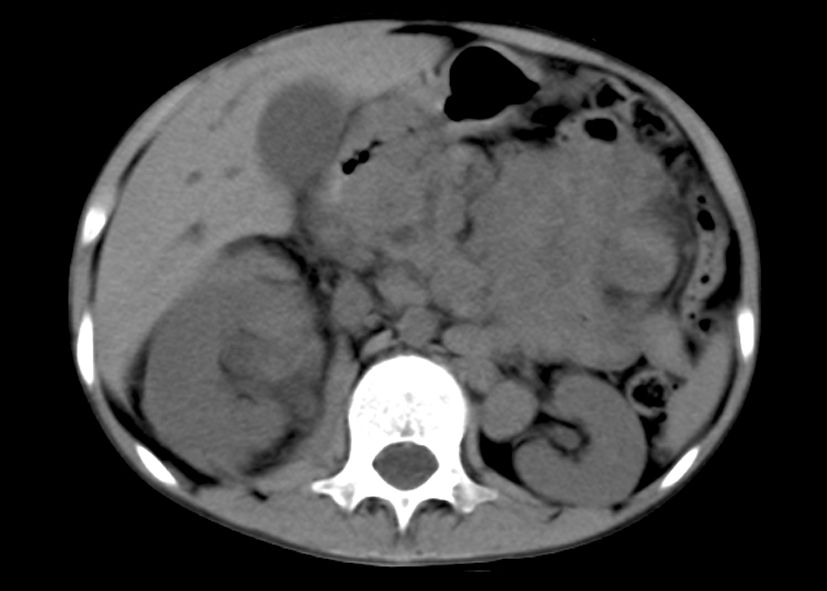
\includegraphics[width=.7\textwidth,height=\textheight,keepaspectratio]{./images/Image00385.jpg}
 \captionsetup{justification=centering}
 \caption{NHL侵及右肾和肠系膜\\{\small 可见腹膜后多个淋巴结增大,腹膜腔巨大肿块,右肾增大、密度减低}}
 \label{fig19-4}
  \end{figure} 

\subsection{腹膜后淋巴结转移瘤}

\textbf{【病理】}
腹膜后转移瘤主要沿腹膜后淋巴系统途径扩散,与原发灶位置及性质有关。不同的肿瘤有一定的优势扩散途径及趋势:①精囊、子宫、卵巢肿瘤比较容易转移到肾门、主动脉旁淋巴结;②胰腺和胃的癌肿易转移到相邻淋巴结;③结肠癌容易转移至肠系膜根部淋巴结;④盆腔肿瘤(包括膀胱、前列腺等)也容易侵犯髂区、骶前淋巴结;⑤比较晚期的病例,下腔静脉、腹主动脉都可能被转移瘤所包绕。

\textbf{【CT表现】}
对腹膜后的转移瘤,应注意从近到远,从原发到转移,全面观察、综合判断。淋巴转移多位于腹主动脉旁淋巴结。增大的淋巴结可呈单一或多个类圆形软组织结节影,边缘清楚。多个增大淋巴结可融合成分叶状肿块,推移或包绕大血管,部分淋巴结可发生坏死而致密度不均。增强扫描可呈轻度至明显均一或不均一强化(图\ref{fig19-5})。偶可呈环状强化,应注意与结核相鉴别。

\begin{figure}[!htbp]
 \centering
 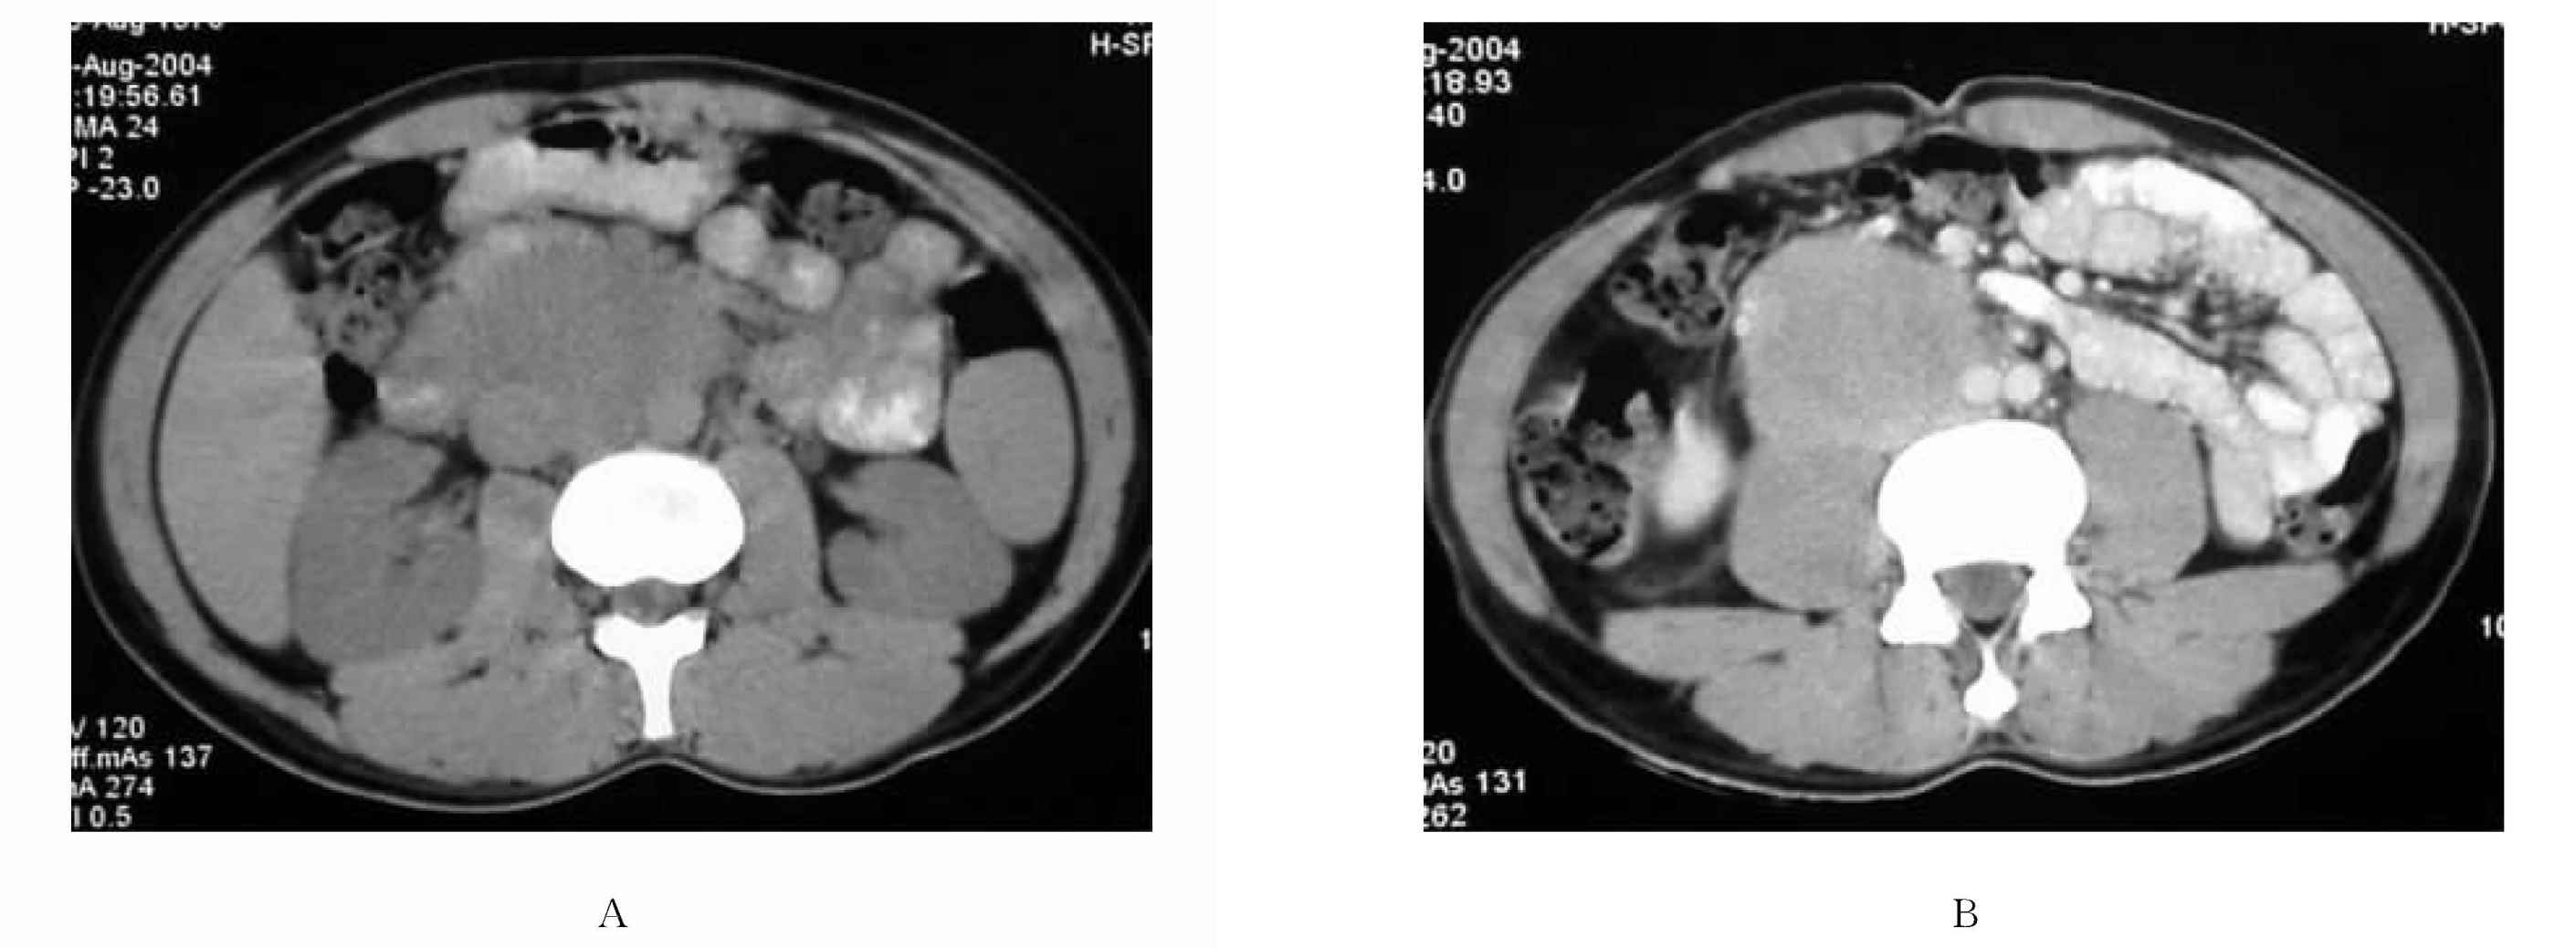
\includegraphics[width=.7\textwidth,height=\textheight,keepaspectratio]{./images/Image00386.jpg}
 \captionsetup{justification=centering}
 \caption{腹膜后淋巴结转移瘤\\{\small 来源于睾丸癌,A、B分别为平扫和增强扫描,腹膜后有许多增大淋巴结并融合成巨大团块}}
 \label{fig19-5}
  \end{figure} 

\subsection{盆部淋巴结的少见病变}

1.巨淋巴结增生症:以纵隔多见,在腹、盆部约占11%,以透明血管型多见,占80%~90%。因其血供丰富,CT表现均匀显著强化,CT值增加40Hu以上。本病常为单发,或为一个特大的淋巴结周围伴形态相同的卫星结节。与淋巴瘤常为多个区域淋巴结增大有别,其表现与结核等亦有别,但需注意排除转移瘤。

2.恶性组织细胞增生症:最易受累的器官为淋巴结、肝脏、脾脏和骨髓,以及肺、肾和心脏等。CT表现为多组淋巴结增大,肝、脾增大等并结合临床检验可以考虑,确诊有赖于病理。

3.血管免疫母细胞淋巴结病:本病为潜在恶性,30%可转化为恶性淋巴瘤,可有全身淋巴结增大、发热、肝脾大、贫血等特点。难与淋巴瘤鉴别,确诊有赖于病理。

4.白血病:引起淋巴结增大多见于慢性和急性淋巴细胞性白血病,可有腹部弥漫性淋巴结增大及肝脾肿大,需结合实验室检查确诊。

5.结节病:腹部表现为淋巴结增大,甚至广泛性增大。肝、脾内可有多发低密度。

\section{腹膜后纤维化及腰肌病变}

\subsection{腹膜后纤维化}

本病命名混乱,如Ormond病、非特异性腹膜后炎、硬化性腹膜后炎、腹膜后炎伴血管周围纤维化以及主动脉周围炎等。

\textbf{【病因】}
本病2/3为特发性,1/3为继发性,恶性约占8%~10%。目前多认为本病与机体对粥样硬化物的自身免疫反应有关。特发性通常只发生于肾门水平至髂动脉分叉的腹主动脉周围,多伴有明显的主动脉粥样硬化。特发性者可合并硬化性胆管炎、Reidel甲状腺炎、Crohn病、动脉炎等全身疾病,可伴发系统性红斑狼疮、眼非肉芽肿型全葡萄膜炎等,提示本病与这些免疫性疾病有关。继发性可能与长期摄入甲基麦角类药物有关,其次与应用β受体阻止剂、甲基多巴、肼酞嗪及一些止痛药、抗生素有关,顺铂化疗所致亦有报道。也可能与动脉瘤及主动脉瘤手术、放疗等因素,以及结核、梅毒、放线菌等特殊感染有关。恶性者多来自恶性肿瘤转移。

\textbf{【病理】}
为灰白色的纤维斑块,由不同成熟度的细胞和纤维化组织构成。初期主要为大量成纤维细胞、炎性细胞浸润及毛细血管增生。成熟后主要为纤维化伴肿块的收缩,细胞成分明显减少。恶性斑块除上述病理表现外,可见散在恶性细胞。

\textbf{【临床表现】}
本病罕见,以白种人多见。发病率为1/20万。好发于30~60岁男性,男性为女性的1~2倍。临床症状多趋向于隐匿性。患者可有非特异的背痛、腹痛、全身不适和体重下降,实验室检查血沉增快。常累及输尿管引起尿路梗阻,偶见血尿,邻近大血管受累可有相应症状。偶见累及胆道、门静脉系统、纵隔、盆腔等出现相应表现。

\textbf{【CT表现】}
①纤维斑块位于肾门至腹主动脉分叉水平,病灶以腹主动脉为中心,位于其前方及两侧,背侧少见。②其前界一般为后腹膜,界限清楚;后界界限不清。可包绕腹主动脉、下腔静脉、髂总静脉及输尿管。外界位居输尿管外侧,但不超过其1cm,故腰大肌的边缘多清晰。③因肿块多不伸向主动脉后方,故主动脉多无前移,但也有个别报道主动脉前移。④输尿管因纤维收缩而多内移。⑤主动脉偶可扩张。⑥腹主动脉或下腔静脉及其分支狭窄、闭塞和(或)静脉内血栓形成多需造影确诊。⑦如病灶累及肝门、十二指肠、乙状结肠、直肠及子宫等出现相应外压性表现,但易误为肿瘤。⑧增强扫描示病灶呈不同密度的斑片状或均匀强化,亦可强化不明显。强化明显者可与腹主动脉CT值相近,动态观察可见病灶增强时间长,延迟5分钟左右其CT值高于腹主动脉。病灶强化程度反映了病灶内的毛细血管含量,也反映了病灶的成熟程度(图\ref{fig19-6})。

\begin{figure}[!htbp]
 \centering
 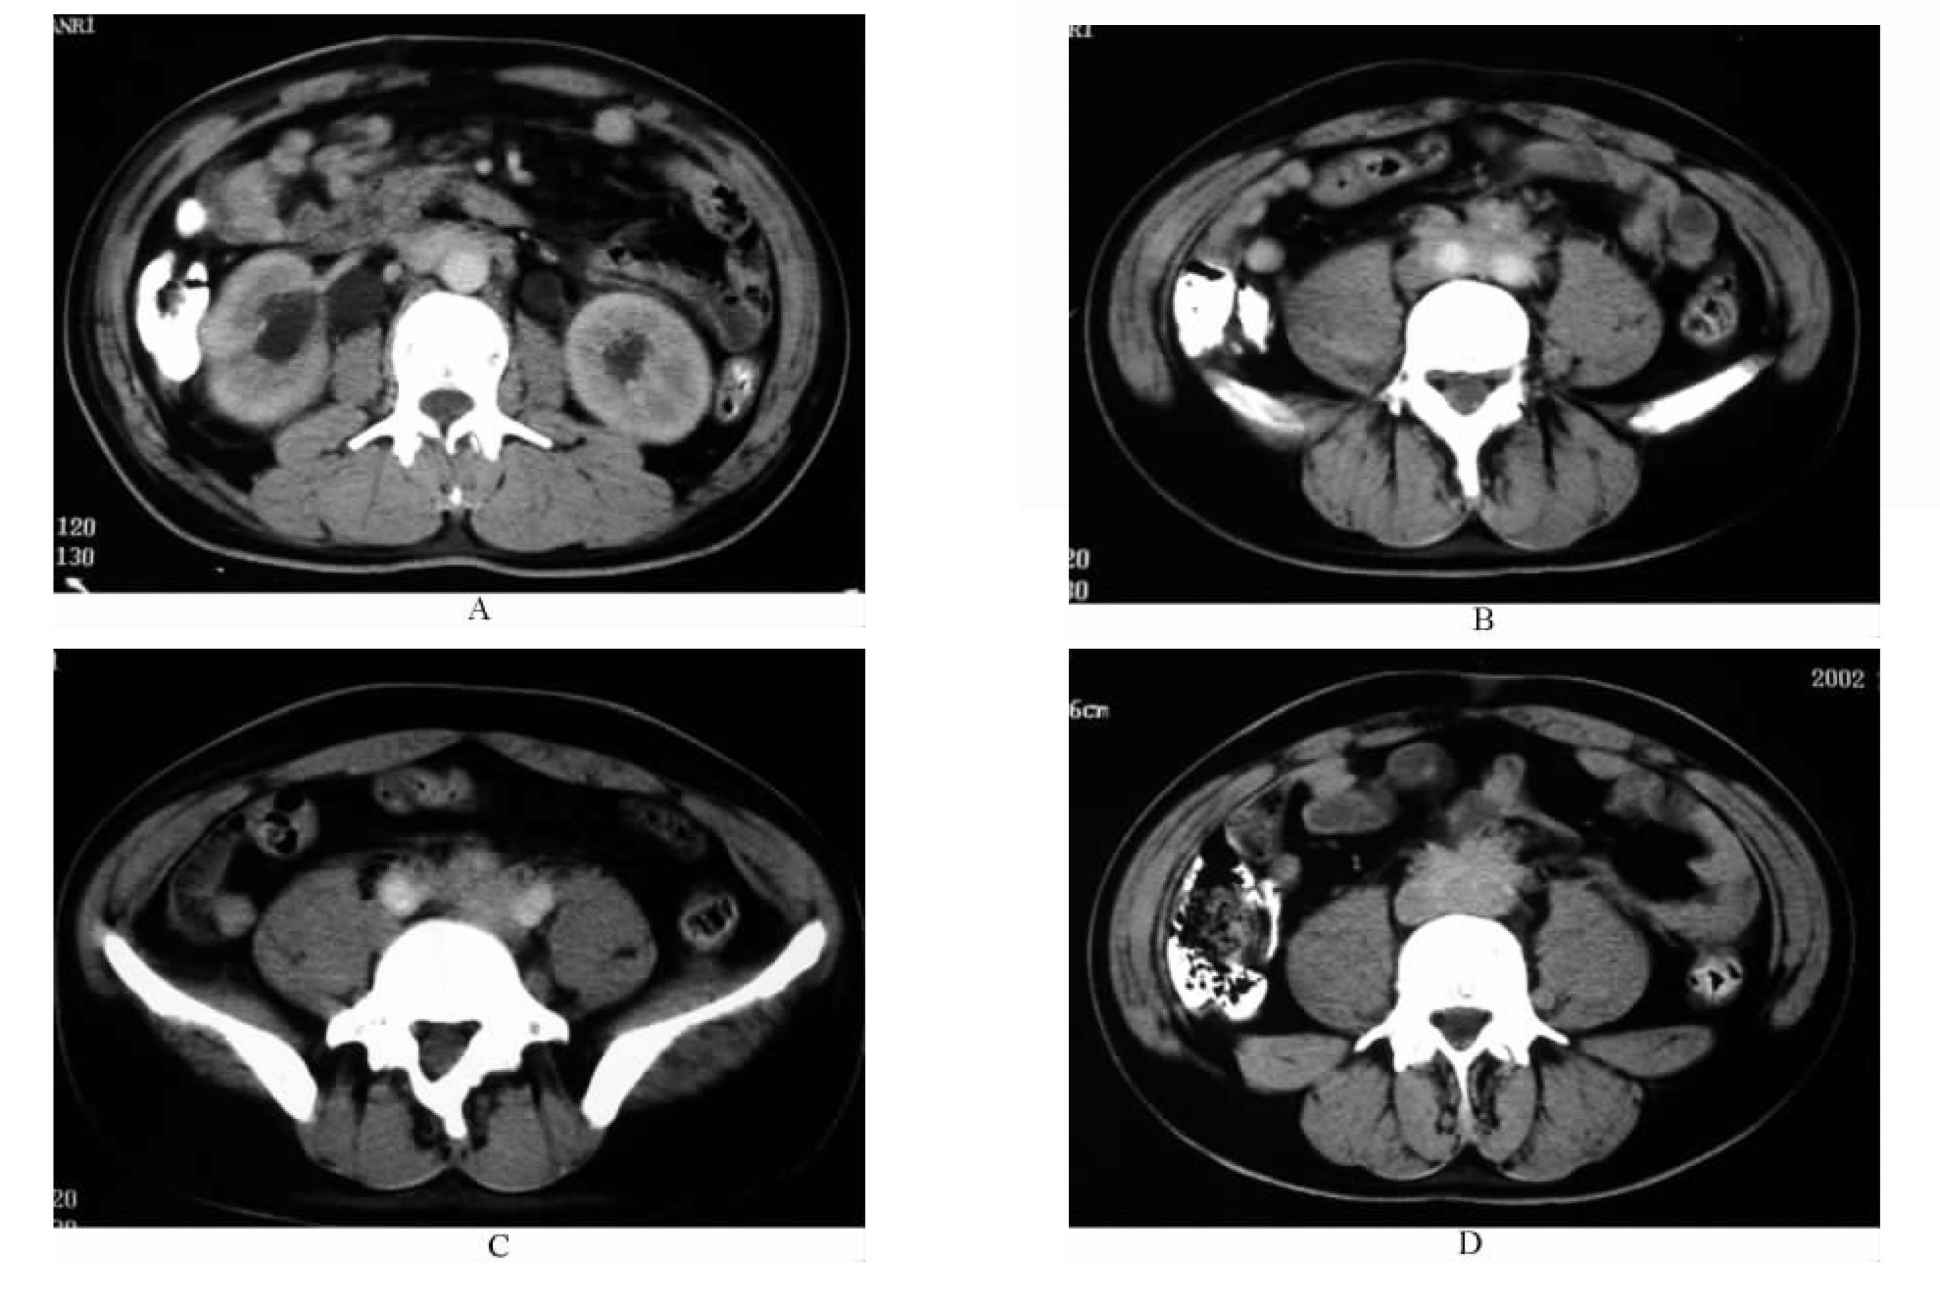
\includegraphics[width=.7\textwidth,height=\textheight,keepaspectratio]{./images/Image00387.jpg}
 \captionsetup{justification=centering}
 \caption{腹膜后纤维化\\{\small A~D为同一患者增强扫描,肾门至腹主动脉分叉水平有不规则软组织密度灶,包绕腹主动脉和下腔静脉,外缘至输尿管区;病灶有欠均匀强化,D示延迟7分钟扫描其CT值高于腹主动脉}}
 \label{fig19-6}
  \end{figure} 

\textbf{【鉴别诊断】}
该病主要应与淋巴瘤和转移性淋巴结增大相鉴别。CT显示的下述特点有助于鉴别,也是良、恶性腹膜后纤维化的鉴别依据。①斑块分布于肾门至腹主动脉分叉水平;②斑块主要位于主动脉前方和两侧且不超过腰大肌;③斑块外形可不规则,但无结节融合或分叶状;④相邻骨及其他组织受压,但无侵蚀破坏。

其他还需与淀粉样变、腹膜后血肿及炎症鉴别。纤维斑块位于盆腔,累及胆道、门静脉以及胰腺等易误诊。

\subsection{腰肌脓肿}

\textbf{【病因】}
腰肌病变中最常见的是感染性疾病,通常是从邻近结构如脊椎、肾、胰腺或肠袢的感染灶直接蔓延而来。常见的病因是结核和化脓性感染。病灶主要累及腰大肌,属于腹肌后群的腰方肌亦可受累。

\textbf{【临床表现】}
因原发病变的病因不同而其临床表现各异,如出现急性感染症状或结核中毒症状。此外,可能触及由腰大肌或髂肌脓肿所致的腹部包块。

\textbf{【CT表现】}
受累的腰肌常弥漫性增大,密度不均,可伴病灶中心低密度坏死灶,CT值约0~30Hu。慢性脓肿壁可有钙化,增强扫描脓肿的周边强化。如在包块内发现气泡或液平面,则有助于腰肌脓肿的诊断(图\ref{fig19-7})。如在脓肿内见到散在钙化,则高度提示结核性冷脓肿。由于原发性腰肌脓肿十分罕见,故应注意邻近结构有无原发病变。

\begin{figure}[!htbp]
 \centering
 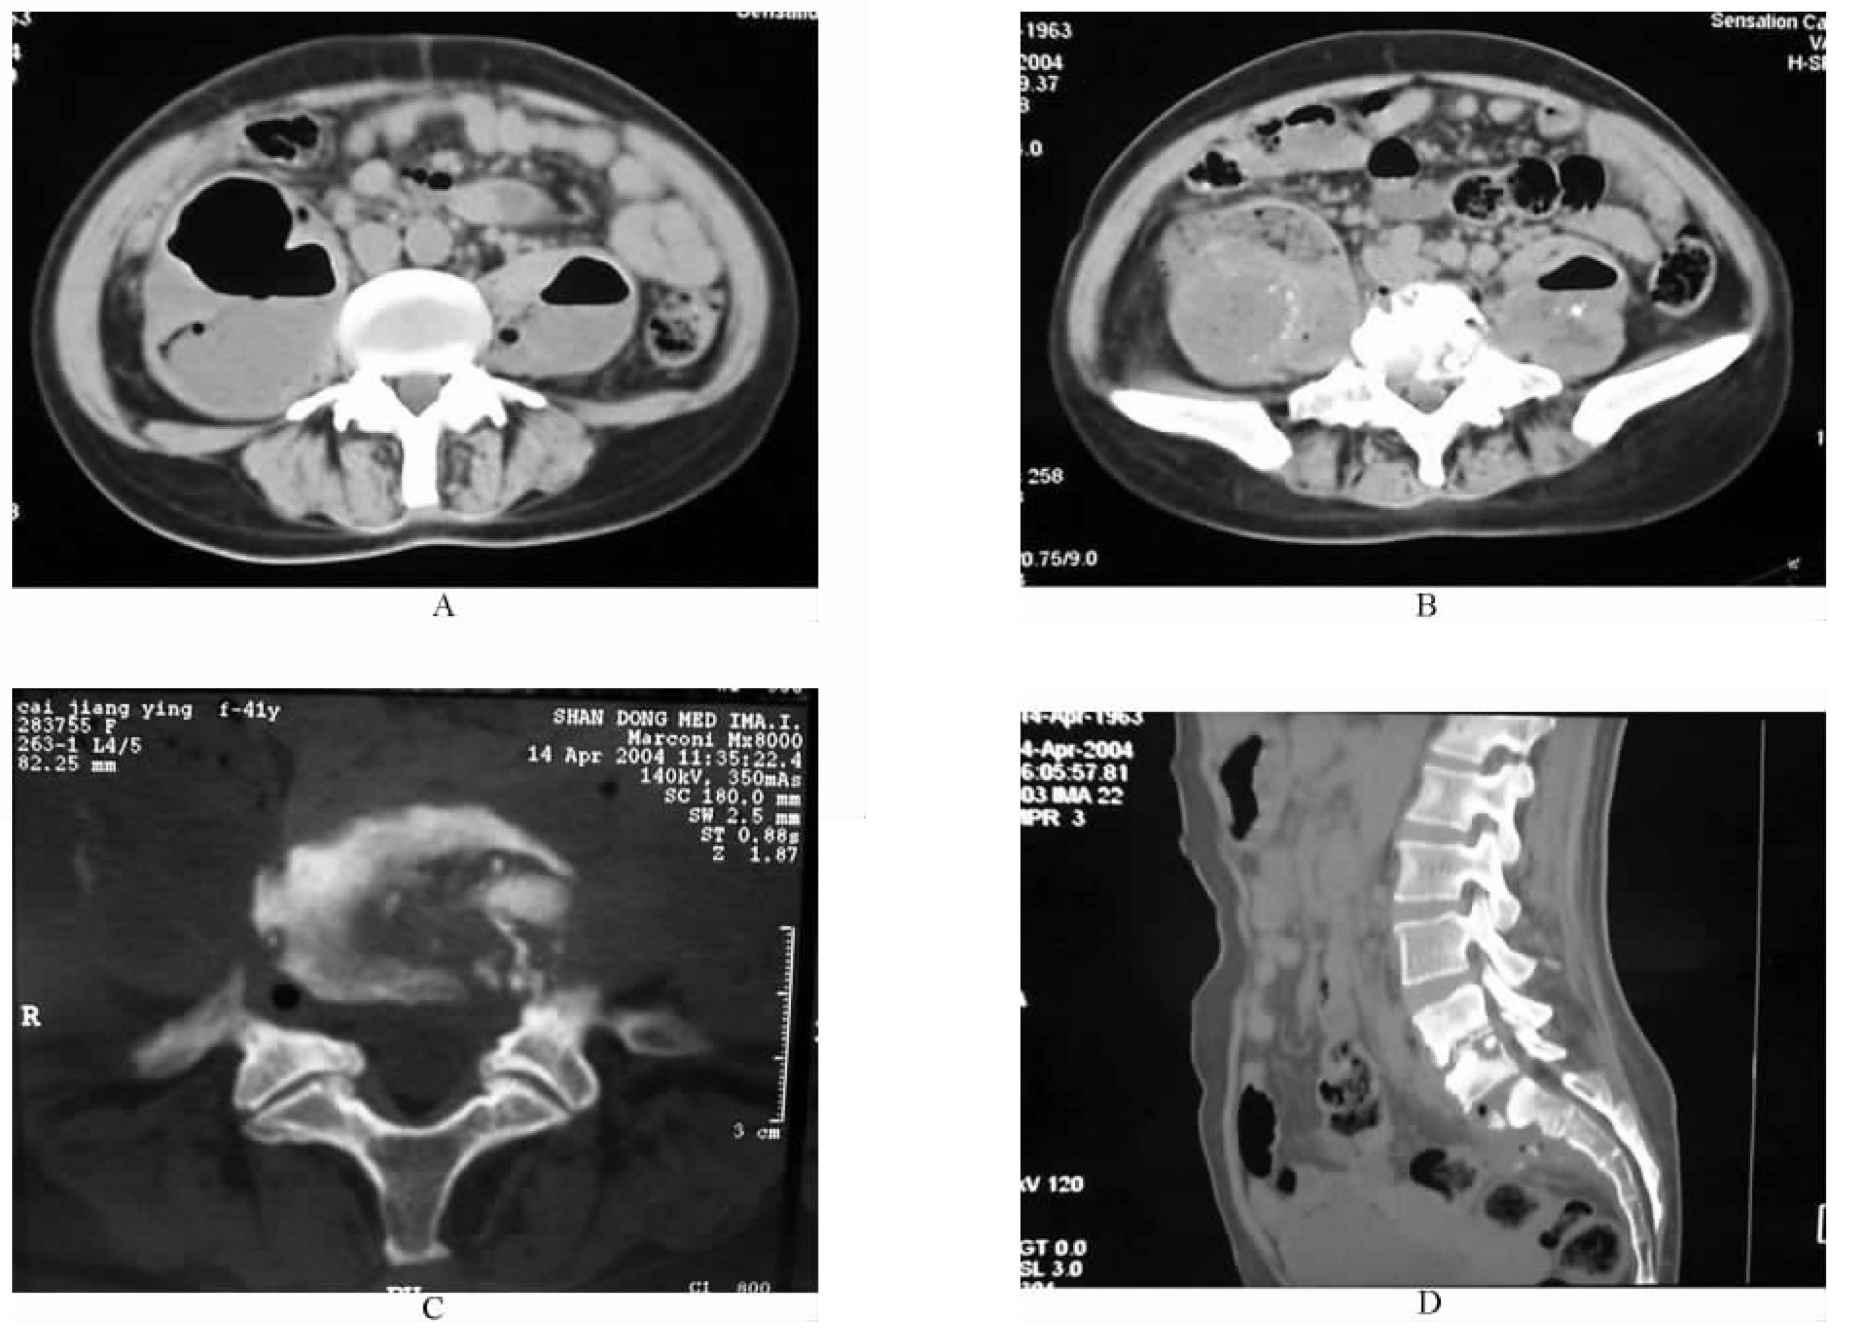
\includegraphics[width=.7\textwidth,height=\textheight,keepaspectratio]{./images/Image00388.jpg}
 \captionsetup{justification=centering}
 \caption{左右腰大肌结核性脓肿\\{\small A~D为同一患者,A、B显示脓肿,脓腔内有液气平面并有钙化,C、D显示腰椎结核表现}}
 \label{fig19-7}
  \end{figure} 

\subsection{腰肌血肿}

\textbf{【病因】}
外伤、出血性疾病、腹主动脉瘤渗漏或破裂可导致腹膜后腔出血,并可产生腰肌血肿或腹后壁血肿。

\textbf{【CT表现】}
受累腰肌体积增大、密度不均,或因反复出血而成分层状。CT值受血肿新鲜程度不同而不等。增强扫描无强化。对于亚急性或慢性腰肌血肿,MR有助于明确诊断。

\subsection{腰大肌肿瘤}

\textbf{【病因病理】}
腰大肌原发性肿瘤比较少见,常为肾脏恶性肿瘤直接侵犯腰大肌或转移性腰大肌肿瘤(如前列腺癌、子宫癌等),还有阑尾黏液囊腺癌侵及腰大肌的报道。肿瘤组织可完全取代肌肉组织,或推移腰肌向内或外侧移位。

\textbf{【临床表现】} 其临床表现较为隐匿,可有腰痛或相应部位发现腹块等。

\textbf{【CT表现】}
患侧腰大肌普遍增大、局部增大或轮廓模糊不清。CT值多与正常肌肉相仿,有时肿瘤中心可出现低密度坏死区。增强扫描可呈不均匀强化。但对转移性肿瘤,应结合临床综合诊断。

\protect\hypertarget{text00027.html}{}{}

